\documentclass{article}

\usepackage{titlesec}
\titleformat{\chapter}[display]
{\normalfont\huge\bfseries}{\chaptertitlename\ \thechapter}{20pt}{\Huge}   
\titlespacing*{\chapter}{0pt}{-50pt}{40pt}

\usepackage[utf8]{inputenc}
\usepackage[T1]{fontenc}
\renewcommand{\familydefault}{\sfdefault}
\usepackage[italian]{babel}

\usepackage[top=20mm, bottom=30mm,
	left=20mm, right=20mm]{geometry}

\usepackage{graphicx}
\usepackage[htt]{hyphenat}

\usepackage{hyperref}
\hypersetup{
	colorlinks=true,
	urlcolor=blue,
	linkcolor=blue,
	citecolor=red
}


\usepackage{color}
\definecolor{mygreen}{rgb}{0,0.6,0}
\definecolor{mygray}{rgb}{0.5,0.5,0.5}
\definecolor{mymauve}{rgb}{0.58,0,0.82}

\usepackage{listings}
\lstset{ 
  backgroundcolor=\color{white},
  basicstyle=\footnotesize,
  breakatwhitespace=false,
  breaklines=true,
  captionpos=b,
  commentstyle=\color{mygreen},
  deletekeywords={...},
  extendedchars=true,
  firstnumber=1000,
  frame=single,
  keepspaces=true,
  keywordstyle=\color{blue},
  language=Java,
  mathescape=true,
  morekeywords={*,...},
  numbers=left,
  numbersep=5pt,
  numberstyle=\tiny\color{mygray},
  rulecolor=\color{black},
  showspaces=false,
  showstringspaces=false,
  showtabs=false,
  stepnumber=2,
  stringstyle=\color{mymauve},
  tabsize=2,
  title=\lstname
}

\usepackage{amsmath}
\usepackage{amssymb}
\usepackage{amsfonts}
\usepackage{amsthm}

\title{Progetto di Tecnologie Web}
\author{Elisa Solinas}
\date{A.A. 2018-2019}

\begin{document}

\pagestyle{empty}


\null\vspace{\stretch{8}}
\centerline {\Large\textsc{Progetto di Tecnologie Web}}

\vskip 3cm

\centerline {\Large{\textsc{Elisa Solinas}}}
\vskip 1cm
\centerline {\Large{\textsc{811737}}}
\vskip 2cm
\centerline
{\Large \url{https://gitlab2.educ.di.unito.it/st159373/t-web}}
\vskip 3cm

\centerline {\Large\textsc{A.A. 2018/2019}}
\vspace{\stretch{10}}\null



\pagebreak

\pagestyle{plain}
\section{Tema del sito}
Il sito realizzato costituisce una piattaforma per l'acquisto di musica heavy metal in formato digitale.\\
La home page del sito presenta una galleria di immagini che mostra le copertine dei dischi più venduti, mentre mediante la barra di navigazione del sito è possibile visualizzare i prodotti appartenenti a un dato genere musicale.\\
L'utente può, inoltre, visualizzare gli acquisti precedentemente effettuati, inserire un prodotto nella "wishlist" e salvarlo per un acquisto successivo, oppure acquistarlo immediatamente.
\section{Le sezioni principali}
\begin{itemize}
    \item \textbf{Accesso al sito}: mediante la pagina di accesso, l'utente può effettuare il login oppure la registrazione. In quest'ultimo caso, i suoi dati verranno inseriti nel database e il login verrà effettuato automaticamente. 
    \item \textbf{Home page}: da questa pagina, l'utente può visualizzare i prodotti più venduti.
    \item \textbf{Navigazione per genere}: questa pagina permette di visualizzare tutti gli album del genere selezionato.
    \item \textbf{Pagina del prodotto}: questa pagina permette di visualizzare il prodotto selezionato e di acquistarlo (oppure aggiungerlo alla wishlist) trascinando la copertina del disco sull'area appropriata.
    \item \textbf{Prodotti acquistati}: questa pagina permette di visualizzare i prodotti che sono già stati acquistati dall'utente.
    \item \textbf{Wishlist}: questa pagina permette di visualizzare i prodotti che l'utente ha salvato per un eventuale acquisto.
\end{itemize}
\section{Funzionalità}
\begin{itemize}
    \item \textbf{Login}: l'utente effettua il login inserendo la propria email e la password nell'apposito form della pagina iniziale.\\
    Quando l'utente clicca sul bottone \texttt{Login}, viene inviata una richiesta di tipo \texttt{POST} AJAX al server, che verifica che le informazioni fornite siano valide e che corrispondano a quelle presenti nel database e setta la variabile \texttt{\$\_SESSION["user"]}.\\
    A questo punto la funzione JavaScript reindirizza l'utente alla home page del sito.
    \item \textbf{Logout}: l'utente può effettuare il logout in qualsiasi momento, cliccando sul pulsante \texttt{logout} presente nella barra di navigazione.\\
    Al click, viene eseguita la funzione \texttt{php-server/logout.php}, che, dopo aver distrutto le variabili di sessione, reindirizza l'utente alla pagina di accesso al sito.
    \item \textbf{Registrazione}: l'utente si registra inserendo la propria email e una password nell'apposito form della pagina iniziale.\\
    Quando l'utente clicca sul bottone \texttt{Subscribe}, viene inviata una richiesta di tipo \texttt{POST} AJAX al server, che verifica che le informazioni fornite siano valide, inserisce il nuovo utente nel database ed effettua il login (settando la variabile \texttt{\$\_SESSION["user"]}).\\
    A questo punto la funzione JavaScript reindirizza l'utente alla home page del sito.
    \item \textbf{Gestione del contenuto generato dall'utente}: l'utente può organizzare i prodotti a cui è interessato in una wishlist (che viene memorizzata sul database), oppure acquistare immediatamente un prodotto (che viene inserito nello storico dei prodotti acquistati). 
\end{itemize}
\section{Caratteristiche}
\begin{itemize}
    \item \textbf{Usabilità}: il sito è stato realizzato cercando di seguire le linee guida per una buona usabilità. In quest'ottica, si è evitato l'utilizzo di pop-up, messaggi di errore difficili da comprendere per l'utente e assenza di feedback dopo un'azione dell'utente.
    \item \textbf{Interazione/animazione}: l'animazione è stata realizzata nella funzione di aggiunta di un prodotto alla wishlist o di acquisto del prodotto.\\
    L'utente vede a sinistra il prodotto selezionato e a destra, due \textit{"box"} che riportano rispettivamente la dicitura \textit{"Trascina qui per acquistare"} e \textit{"Trascina qui per aggiungere il prodotto alla wishlist"}.\\
    L'utente, mediante drag and drop, trascina la copertina dell'album sul box dell'azione che intende effettuare.
    \item \textbf{Sessioni}: la sessione dell'utente viene aperta mediante login (oppure registrazione) e viene chiusa, dall'utente stesso, mediante il click sul pulsante logout (oppure, come da default per PHP, dopo 24 minuti).
    \item \textbf{Interrogazione del database}: per l'interrogazione del database, effettuata unicamente lato server, è stata usata la classe PDO, in modo da poterne sfruttare le caratteristiche di sicurezza (per evitare gli attacchi di tipo SQL Injection) e di efficienza.\\
    \item \textbf{Validazione dei dati in input}: i dati inseriti dall'utente vengono validati lato client utilizzando i vincoli forniti da HTML5, cioè \texttt{required} e \texttt{type}, che impediscono l'invio del form nel caso in cui i campi non siano stati compilati, oppure i dati inseriti non siano del formato adeguato (in particolare, nel caso in cui l'email inserita non sia valida e/o la password non rispetti la lunghezza minima di 8 caratteri).\\
    Anche lato server si verifica che i campi siano stati compilati, che l'email inserita sia valida e che la password rispetti la lunghezza minima di 8 caratteri, e, inoltre, tutte le query del database che prevedono l'utilizzo di dati inseriti dall'utente vengono realizzate mediante il metodo \texttt{prepare} della classe PDO.
    \item \textbf{Presentazione}: il layout del sito è volutamente aggressivo (testo neon su sfondo nero) in accordo con la tematica del sito e si è utilizzato Bootstrap 4 in modo tale da renderlo responsive.
\end{itemize}
\section{Front-end}
\begin{itemize}
    \item \textbf{Separazione presentazione/contenuto/comportamento}: il codice HTML di ogni pagina del sito (\textbf{contenuto}) è inserito in un file \texttt{\textit{filename}.php}, il quale include come riferimenti il foglio di stile \texttt{style.css} (\textbf{presentazione}) e il file contenente gli script utilizzati dalla pagina, \texttt{\textit{filename}.js} (\textbf{comportamento}).
    \item \textbf{Soluzioni cross-platform}:
        Il sito è stato testato sulle ultime versioni dei seguenti browser:
            \begin{itemize}
                \item Safari
                \item Google Chrome
                \item Firefox
                \item Opera
            \end{itemize}
        Si è fatto affidamento alle funzionalità di jQuery e di Bootstrap 4 per risolvere i problemi di compatibilità con eventuali browser più datati.
    \item \textbf{Organizzazione file e cartelle di progetto}: il progetto è suddiviso nelle seguenti cartelle:
        \begin{itemize}
            \item \texttt{css}: questa cartella contiene il solo file \texttt{style.css}.
            \item \texttt{files}: questa cartella contiene le immagini di copertina degli album presenti nel database.
            \item \texttt{js}: questa cartella contiene i file JavaScript, ciascuno dei quali ha il nome della pagina web che deve eseguirne il codice.
            \item \texttt{librerie}: questa cartella contiene i file dei framework jQuery, Bootstrap (sia CSS che JS) e Popper.js (richiesta da Bootstrap).
            \item \texttt{php-sections}:  questa cartella contiene i file \texttt{php} delle porzioni di codice che vengono riutilizzate più volte dalle pagine (\texttt{head}, \texttt{footer}, e \texttt{navbar}).
            \item \texttt{php-server}: questa cartella contiene i file delle funzioni \texttt{php} che vengono eseguite dal server, compreso il file \texttt{database.php} che include tutte le funzioni di accesso al database.
            \item \texttt{php-views}: questa cartella contiene i file \texttt{php} delle pagine del sito.
        \end{itemize}
\end{itemize}
\section{Back-end}
\begin{itemize}
    \item \textbf{Architettura generale classi/funzioni PHP}: le funzioni PHP vengono richiamate mediante chiamate JavaScript/AJAX e sono inserite all'interno di file che ne portano il nome.\\
    Fanno eccezione le funzioni che hanno il compito di interrogare il database, inserite nel file \texttt{database.php}
    \item \textbf{Schema del database}: 
    	\begin{figure}[h!]
    		\centering
    		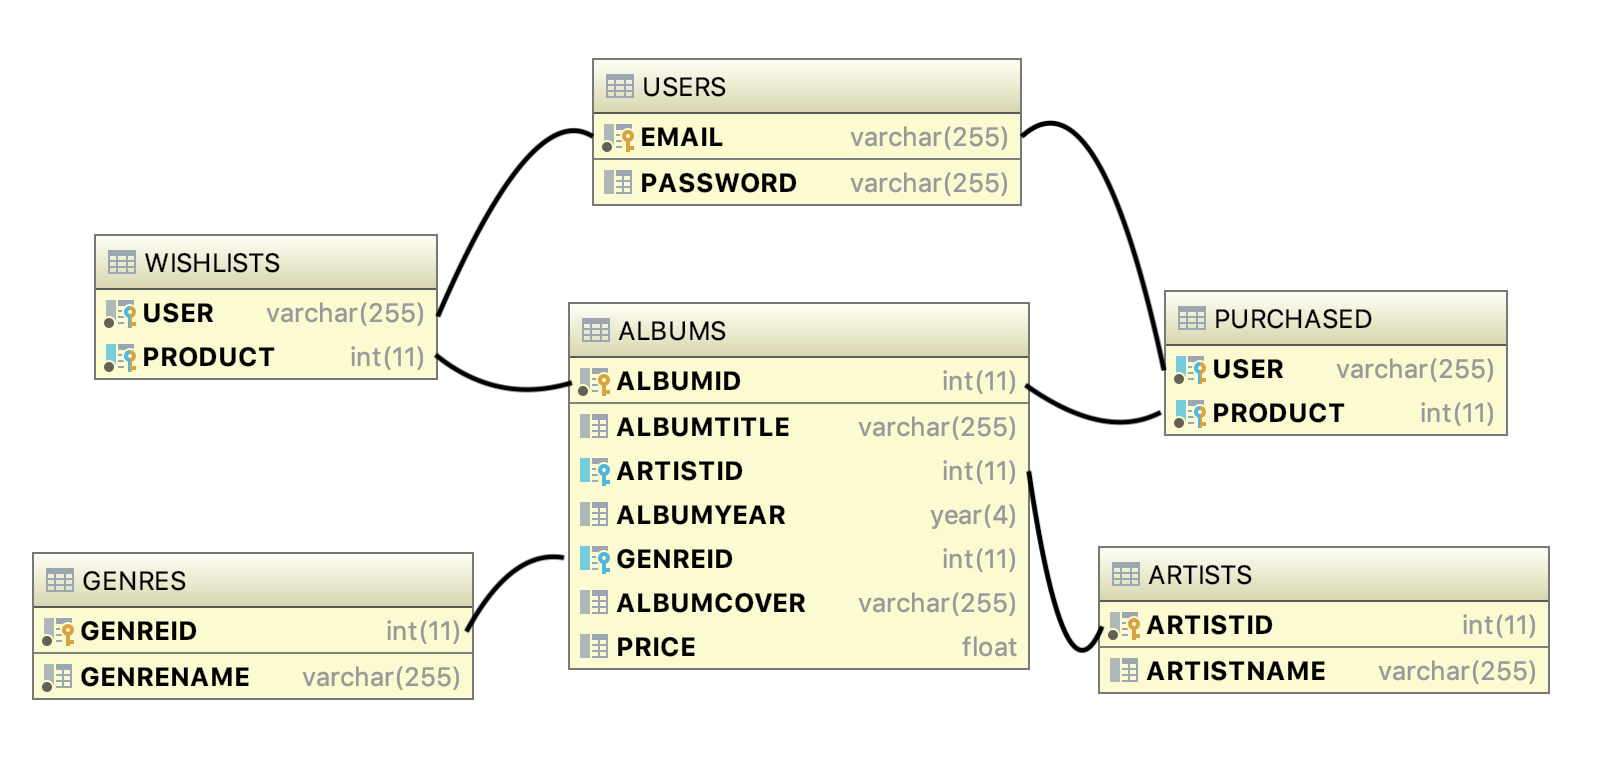
\includegraphics[scale=0.55]{schema-db.png}
    	\end{figure}
    \item \textbf{Descrizione delle funzioni remote}:
        \begin{itemize}
            \item \texttt{add\_to\_purchased.php}: viene invocata quando l'utente acquista un prodotto.\\
            Riceve in input la variabile $\texttt{\$\_POST["album"]}$, che contiene l'id dell'album da inserire tra gli acquisti e utilizza la variabile $\texttt{\$\_SESSION["user"]}$ (se questa non è impostata significa che l'utente non è loggato, quindi si viene reindirizzati alla pagina di accesso).\\
            Invia una richiesta al database che inserisce il prodotto tra gli acquistati e restituisce (in formato JSON), in caso di successo, il codice 200 alla richiesta AJAX, in caso di fallimento , il codice 404 con un messaggio di errore.
            \item \texttt{add\_to\_wishlist.php}: viene invocata quando l'utente inserisce un prodotto nella sua wishlist.\\
            Riceve in input la variabile \texttt{\$\_POST["album"]}, che contiene l'id dell'album e utilizza la variabile \texttt{\$\_SESSION["user"]} (se questa non è impostata significa che l'utente non è loggato, quindi si viene reindirizzati alla pagina di accesso).\\
            Invia una richiesta al database che inserisce il prodotto nella wishlist e restituisce (in formato JSON), in caso di successo, il codice 200, in caso di fallimento , il codice 404 con un messaggio di errore.
            \item \texttt{delete\_from\_wishlist.php}: viene invocata quando l'utente clicca sul bottone \texttt{Delete} dalla pagina che mostra la wishlist.\\
             Riceve in input la variabile \texttt{\$\_POST["album"]}, che contiene l'id dell'album e utilizza la variabile \texttt{\$\_SESSION["user"]} (se questa non è impostata significa che l'utente non è loggato, quindi si viene reindirizzati alla pagina di accesso).\\
            Invia una richiesta al database che rimuove il prodotto dalla wishlist e restituisce (in formato JSON), in caso di successo, il codice 200 e la copia della wishlist aggiornata, in caso di fallimento , il codice 404 con un messaggio di errore.
            \item \texttt{get\_album.php}: viene invocata quando l'utente clicca su un album per visualizzarne i dettagli.\\
            Riceve in input la variabile \texttt{\$\_POST["album"]}, che contiene l'id dell'album (se questa non è impostata viene restituito un messaggio di errore). 
            Il server interroga il database per ottenere tutti i dettagli sull'album (viene generato un messaggio di errore anche nel caso in cui l'album selezionato non sia presente) e restituisce le informazioni ricavate (in formato JSON) nel caso in cui la ricerca sia andata a buon fine.
            \item \texttt{get\_bestsellers.php}: questa funzione restituisce, in formato JSON, gli album più venduti presenti nel database.\\
            In caso di errore, viene generato un messaggio che informa l'utente.
            \item \texttt{get\_by\_genre.php}: riceve in input la variabile \texttt{\$\_POST["genre"]}, che contiene l'id del genere musicale selezionato dall'utente (se questa non è impostata viene restituito un messaggio di errore) e, interrogando il database, restituisce la lista degli album di tale genere in formato JSON.\\
            Nel caso in cui si verifichi un errore, viene generato un messaggio che informa l'utente.
            \item \texttt{get\_genres.php}: questa funzione restituisce una lista, in formato JSON, di tutti i generi presenti nel database. \\
            Nel caso in cui si verifichi un errore, viene generato un messaggio che informa l'utente.
            \item \texttt{get\_purchased.php}: utilizzando la variabile \texttt{\$\_SESSION["user"]}, resituisce la lista degli album acquistati dall'utente. \\
            Se la variabile \texttt{\$\_SESSION["user"]} non è impostata significa che l'utente non è loggato, quindi si viene reindirizzati alla pagina di accesso.\\
            Nel caso in cui si verifichi un errore, viene generato un messaggio che informa l'utente.
            \item \texttt{get\_wishlist.php}: utilizzando la variabile \texttt{\$\_SESSION["user"]}, resituisce la lista degli album che l'utente ha inserito nella sua wishlist. \\
            Se la variabile \texttt{\$\_SESSION["user"]} non è impostata significa che l'utente non è loggato, quindi si viene reindirizzati alla pagina di accesso.\\
            Nel caso in cui si verifichi un errore, viene generato un messaggio che informa l'utente.
            \item \texttt{login.php}: questa funzione riceve in input le variabili \texttt{\$\_POST["email"]} e \texttt{\$\_POST["password"]} e ne verifica la validità.\\
            Nel caso in cui si verifichi un errore, viene generato un messaggio che informa l'utente.
            \item \texttt{logout.php}: questa funzione riceve in input la variabile \texttt{\$\_SESSION["user"]}, distrugge le variabili di sessione e reindirizza l'utente alla pagina di accesso al sito.\\
            Nel caso in cui si verifichi un errore, viene generato un messaggio che informa l'utente.
            \item \texttt{subscribe.php}: questa funzione riceve in input le variabili \texttt{\$\_POST["email"]} e \texttt{\$\_POST["password"]}, ne verifica la validità e verifica che l'utente non sia presente nel database.\\
            Nel caso in cui si verifichi un errore, viene generato un messaggio che informa l'utente.
        \end{itemize}
    \item \textbf{Gestione delle condizioni di errore}: le condizioni di errore vengono gestite come segue:
    	\begin{itemize}
    		\item Errore nella connessione al server o nella chiamata AJAX: l'utente viene reindirizzato alla pagina di accesso al sito, dove visualizza un messaggio di errore che lo invita a riprovare.
    		\item Errore nell'input dei dati: viene visualizzato un messaggio all'interno del form che spiega l'errore commesso.
    	\end{itemize}
    \item \textbf{Funzioni di callback lato Javascript/AJAX}:
        \begin{itemize}
            \item \texttt{add\_to\_purchased}: questa funzione (richiesta di tipo \texttt{GET}) viene invocata nel momento in cui l'utente trascina la copertina dell'album da acquistare nell'apposita area, e richiede al server l'aggiunta dell'album agli acquisti.\\
            Il server risponde indicando il successo o il fallimento dell'operazione.
            \item \texttt{add\_to\_wishlist}: questa funzione (richiesta di tipo \texttt{GET}) viene invocata nel momento in cui l'utente trascina la copertina dell'album da acquistare nell'apposita area, e richiede al server l'aggiunta dell'album alla wishlist.\\
            Il server risponde indicando il successo o il fallimento dell'operazione.
            \item \texttt{delete\_from\_wishlist}: questa funzione viene invocata nel momento in cui l'utente clicca sul pulsante \texttt{Delete} di un elemento della wishlist.\\
            Viene inviata una richiesta al server (di tipo \texttt{POST}), includendo l'ID dell'album da cancellare, e il server risponde con una copia della wishlist aggiornata, che viene ricaricata su schermo.\\
            In caso di errore, l'utente viene informato con un messaggio.
            \item \texttt{get\_album}: questa funzione permette di visualizzare i dettagli di album.\\
            Viene inviata una richiesta al server (di tipo \texttt{POST}), includendo l'ID dell'album e il server risponde con le informazioni richieste.\\
            In caso di errore, l'utente viene informato con un messaggio.
            \item \texttt{get\_bestsellers}: questa funzione permette di visualizzare gli album più venduti.\\
            Viene inviata una richiesta al server (di tipo \texttt{GET}), e il server risponde (in caso di successo) con le informazioni richieste.\\
            In caso di errore, l'utente viene informato con un messaggio.
            \item \texttt{get\_by\_genre}: questa funzione permette di visualizzare tutti gli album di un dato genere.\\
            Viene inviata una richiesta al server (di tipo \texttt{POST}), inviando l'ID del genere selezionato, e il server risponde (in caso di successo) con la lista richiesta.\\
            In caso di errore, l'utente viene informato con un messaggio.
            \item \texttt{get\_genres}: questa funzione viene invocata nel momento in cui viene caricata la barra di navigazione e permette di popolare il menu dropdown con i generi presenti nel database.\\
            Si tratta di una richiesta di tipo \texttt{GET}, che restituisce la lista in caso di successo e un messaggio di errore in caso di fallimento.
            \item \texttt{get\_purchased}: questa richiesta (di tipo \texttt{GET}) riceve la lista degli album acquistati da un dato utente, in caso di successo, mentre in caso di fallimento restituisce un messaggio di errore. 
            \item \texttt{get\_wishlist}:questa richiesta (di tipo \texttt{GET}) riceve la wishlist di un dato utente, in caso di successo, mentre in caso di fallimento restituisce un messaggio di errore. 
            \item \texttt{login}: questa richiesta invia al server (mediante \texttt{POST}) l'email e la password inseriti dall'utente: in caso queste non siano valide (non esiste alcun utente con tale email o la password non è quella giusta per quell'utente), il server risponde con un messaggio di errore. Nel caso, invece, la richiesta vada a buon fine, l'utente viene reindirizzato alla home page del sito.
            \item \texttt{subscribe}: questa richiesta invia al server (mediante \texttt{POST}) l'email e la password inseriti dall'utente: in caso queste non siano valide (la password non è valida oppure esiste già un utente con tale indirizzo email), il server risponde con un messaggio di errore. Nel caso, invece, la richiesta vada a buon fine, l'utente viene reindirizzato alla home page del sito. 
        \end{itemize}
\end{itemize}

\end{document}